%Author: Erik Belko - xbelko02

\documentclass[a4paper, 12pt]{article}[25.11.2020]

\usepackage{times}
\usepackage[left=1.5cm, text={17.5cm, 24cm}, top=3cm]{geometry}
\usepackage[utf8]{inputenc}
\usepackage[slovak]{babel}
\usepackage{graphics}
\graphicspath{ {img/} }
\usepackage{url}
\usepackage{pdflscape}
\usepackage{indentfirst}


\begin{document}


\begin{titlepage}
	\begin{center}
		\Huge \textsc{Vysoké učení technické v Brně} \\
		\vspace{\stretch{0.02}}
		\scalebox{0.3}{
\includegraphics{logo.png}} \\
		\vspace{\stretch{0.362}}
		\Huge{\uppercase{\textbf{Projektová dokumentácia}}} \\
		\LARGE{Implementácia prekladača imperatívneho jazyka IFJ20} \\
		\Large{\verb|Tým 098, varianta II|}
		\vspace{\stretch{0.618}}
	\end{center}
	{\Large \begin{tabular}{l l c}
				\textbf{Harvan Mário} & \verb|xharva03| & \quad 25\,\% \\
				Martiček Juraj & \verb|xmarti97| & \quad 25\,\% \\
				Belko Erik & \verb|xbelko02| & \quad 25\,\% \\
				Šlesár Michal & \verb|xslesa01| & \quad 25\,\% \\
			\end{tabular}
	    \hfill
	\today}
\end{titlepage}

\tableofcontents %kvoli tomuto to bude treba prelozit dvakrat !!!!
\newpage

\section{Úvod}
    \par Cieľom dokumentácie je opísanie implementácie a~postupu pri~riešení projektu
    v~predmetoch IFJ a~IAL. Základ projektu bola implementácia prekladača (program 
    v~jazyku C). Prekladač načíta zdrojový kód zo~zdrojového imperatívneho jazyka
    IFJ20. Jazyk IFJ20 je podmnožinou jazyka GO. Prekladač preloží načítaný kód
    do~cieľového jazyka IFJcode20 a~vypíše na~štandardný výstup alebo sa program
    ukončí s~danou chybovou hláškou.
    
\section{Práca v~tíme}
    \par S~prácou na~prekladači sme začali pomerne skoro kvôli rozsiahlosti projektu.
    Prácu sme si delili rovnomerne počas riešenia projektu. Na úlohách sme väčšinou
    pracovali vo~dvojiciach alebo jednotlivo. Využili sme princípy metodiky Scrum 
    a~prácu sme si rozdelili na~týždňové sprinty.
    \subsection{Komunikácia v~tíme}
        \par Keďže sme sa kvôli momentálnej situácii s~pandémiou nemohli stretávať
        museli sme naplno využiť online komunikačné kanály. Na~komunikáciu v~tíme sme
        využili Discord, na~ktorom sme si vytvorili server. Bol rozdelený na~viacero
        kanálov a~skladov materiálov pre~jednotlivé časti projektu. Využili sme najmä
        voice kanály pre rýchlejšiu a~pohotovejšiu komunikáciu pri~riešení problémov.
        \par Každý týždeň sme telefonovali, zhodnocovali vykonanú prácu a~plánovali si
        úlohy na~další týždeň. Na~plánovanie úloh sme využili software Jira, 
        a~prepojili ho aj s~Discordom.
    \subsection{Verzovací systém}
        \par Pre~správu súborov sme sa rozhodli používať verzovací systém GitLab.
        GitLab nám umožnil pracovať na~projekte súčasne v~tzv. vetvách. Vyplatilo sa
        nám to aj ak sme sa chceli k~niečomu vrátiť a~použiť staršiu verziu. Pracovali
        sme vo~vedlajších vetvách a~až po~schválení úprav ostatnými členmi týmu sme
        úpravy pridali do~hlavnej vetvy vývoja.
\newpage
    \subsection{Rozdelenie práce}
        \subsubsection{Harvan Mário}
            \begin{itemize}
                \item Vedenie tímu a~organizácia práce
                \item Návrh a~implementácia syntaktickej analýzy výrazov
                \item Návrh a~implementácia sémantickej analýzy výrazov
                \item Implementácia zásobníku
            \end{itemize}
        \subsubsection{Martiček Juraj}
            \begin{itemize}
                \item Tvorba tabuľky pre~precedenčnú analýzu
                \item Implementácia dátového typu Vector
                \item Tvorba knižnice pre~error handling a~chybové hlášky
                \item Tvorba generátora kódu
            \end{itemize}
        \subsubsection{Belko Erik}
            \begin{itemize}
                \item Tvorba pravidiel a~tabuľky LL(1) gramatiky
                \item Návrh a~implementácia syntaktickej analýzy (okrem výrazov)
                \item Návrh a~implementácia sémantickej analýzy (okrem výrazov)
                \item Tvorba dokumentácie
            \end{itemize}
        \subsubsection{Šlesár Michal}
            \begin{itemize}
                \item Návrh a~implementácia lexikálnej analýzy
                \item Návrh a~implementácia syntaktickej analýzy (okrem výrazov)
                \item Návrh a~implementácia sémantickej analýzy (okrem výrazov)
                \item Implementácia string knižnice
            \end{itemize}
        \subsubsection{Spoločná práca}
            \begin{itemize}
                \item Testovanie kódu
                \item Tvorba prezentácie
            \end{itemize}

\newpage
\section{Návrh a~implementácia}
    \par Štruktúru projektu, ktorá je popísaná v~tejto časti, ako aj použité algoritmy
    sme zostavili podľa odporúčaní a~návrhov z~prednášok predmetov IFJ a~IAL.
    \subsection{Lexikálna analýza}
        \par Pri~tvorbe prekladača sme začali práve lexikálnou analýzou alebo inak
        povedané scannerom. Scanner načítava znaky zo~zdrojového súboru, vyhodnocuje 
        a~prevádza ich na~tokeny.
        \par Scanner je implementovaný ako deterministický konečný automat. Hlavnou
        funkciou scanneru je funkcia \verb|scanner_get_token|, ktorá spracováva
        načítané znaky a~prevádza ich na~štruktúru \verb|token|. Štruktúra
        \verb|token| sa skladá zo~štruktúr \verb|tokenType| pre~typ tokenu a~\verb|tokenValue|
        pre~hodnotu tokenu. Typmi tokenu môžu byť \verb|EOF|, \verb|EOL|, identifikátor,
        kľúčové slovo, prázdny token, čiarka, zátvorky, čísla, reťazce, operátory a~daľšie
        znaky, ktoré sú povolené v~jazyku IFJ20. Hodnota tokenu je \verb|union|, a~podla typu
        tokenu to môže byť reťazec, ak je typ tokenu identifikátor alebo reťazec, int64 alebo
        double, ak sa jedná o~typ tokenu integer číslo alebo float číslo, a~nakoniec typ
        klúčového slova ak bol typ tokenu kľúčové slovo. 
        \par Celý scanner sa skladá z~dlhej série \verb|if|-ov vo~\verb|while| cykle.
        Každý \verb|if| zodpovedá jednému stavu v~konečnom automate. Ak scanner práve
        nájde znak ktorý nezodpovedá jazyku IFJ20 vráti chybu 1. Funkcia
        \verb|scanner_get_token| je ukončená úspešne ak je z~načítaných znakov hotový
        jeden token. Scanner končí s~načítavaním tokenov pokiaľ je ukončený chybou
        alebo ak už prečíta celý zdrojový súbor.
        \par Scanner je implementovaný v~súbore \verb|scanner.c| a~využíva hlavičkový súbor
        \verb|scanner.h|.
    \subsection{Syntaktická analýza}
        \par Po~implementácii lexikálnej analýzy sme začali pracovať na~syntaktickej.
        Syntaktická analýza je jedna z~najdôležitejších častí prekladača, keďže kontroluje
        syntax zdrojového kódu. Syntax je kontrolovaná na~základe LL(1) gramatiky, ktorú sme si
        zostavili ešte pred~implementáciou syntaktickej analýzy. Pre~syntaktickú analýzu sme si
        vybrali spôsob rekurzívneho zostupu. Syntaktická analýza je spolu so~sémantickou
        analýzou implementovaná v~súbore \verb|parser.c|. Parser prechádza zdrojový kód
        dvakrát, kvôli sémantickej analýze. Syntaktická analýza začína funkciou \verb|parse|
        a~postupne cez funkciu \\ \verb|ruleProgram| rekurzívne zostupuje podľa pravidiel LL(1)
        gramatiky a~porovnáva podla nich tokeny. Tokeny získava pomocou funkcie 
        \verb|load_token| od~scanneru alebo zo~zásobníku ak sa tam nejaké nachádzajú. Zásobník 
        sme pri~implementácii použili kvôli pravidlám s~epsilonom. Ak parser narazí na~nejakú
        syntaktickú chybu počas rekurzívneho zostupu, prekladač sa ukončí s~chybou 2. Parser
        využíva aj hlavičkový súbor \verb|parser.h| v~ktorom je okrem iného aj štruktúra
        \verb|ParserData|, v~ktorej sú všetky dáta pre syntaktickú aj sémantickú analýzu. 
        Sú to napríklad \verb|bool isFirstScan| pre~zistenie, či sa práve jedná o~prvý prechod 
        alebo iné využívané štruktúry ako \verb|Vector *scopes|, \verb|htab_t *table|, 
        \verb|Stack *tokens| a~tak ďalej. Osobitnou časťou je syntaktická analýza výrazov, 
        ktorá je implementovaná v~\verb|expression.c| a~popísaná v~časti \ref{expression}.
\newpage
    \subsection{Sémantická analýza}
        \par Spolu so~syntaktickou analýzou je v~\verb|parser.c| implementovaná aj sémantická
        analýza. Sémantická analýza kontroluje sémantické pravidlá podľa zadania a~na to je 
        potrebný dvojitý prechod zdrojového kódu. Parser prechádza zdrojový kód dvakrát, preto
        je potrebné vstup uložiť, my sme zvolili dynamické pole \verb|dynamicArr|. Pri~prvom
        prechode parser kontroluje identifikátory, ukladá si funkcie a~následne pri~druhom 
        prechode sa skontroluje či sú všetky volané funkcie už definované, či neprichádza 
        k~redefinícii, alebo aj to či v~zdrojovom kóde nechýba funkcia main. Sémantická analýza
        kontroluje okrem iného aj správne typy, počet a~návratové hodnoty funkcii, to či sú
        pri~priradeniach premenných premenné už vopred definované. Na~ukladanie premenných sme
        využili systém vytvárania scopov(tabuľka symbolov), k~ich zanorovaniu a~prístupu k~nim
        sme použili štruktúru \verb|Vector|. Posledný prvok vo~Vectore je scope v~ktorom sa
        sémantická analýza práve nachádza, to pomáha sémantickej analýze zisťovať, či sú
        premenné definované v~lokálnom alebo v~niektorom z~vonkajších scopov. Po~prechode
        a~kontrole daného scopu sa scope z~Vectoru odstráni. Implementácia tabuliek symbolov je
        v~\verb|symtable.c| a~popísaná v~časti \ref{symTable}. Sémantická analýza je teda
        so~syntaktickou implementovaná v~rámci rekurzívneho zostupu. Sémantická analýza využíva
        pomocné funkcie z~\verb|semantic_analysis.h|, ktoré využíva aj sémantická analýza
        výrazov, ktorá je implementovaná v~\verb|expression.c| a~popísaná v~časti
        \ref{expression}.
    \subsection{Syntaktická a~sémantická analýza výrazov}\label{expression}
        \par Výrazy spracovávame pomocou precedenčnej analýzy. Keď parser narazí na~miesto
        v~kóde kde očakáva výraz, zavolá funkciu \verb|expression|, ktorá sa nachádza v~súbore
        \verb|expression.c|.
        \par Funkcia \verb|expression| vracia parseru štruktúru \verb|expResult|, ktorá
        obsahuje string \verb|result| obsahujúci názov pomocnej premennej v~ktorej je uložený
        výsledok výrazu, bool \verb|isFunc| ak sme narazili na~volanie funkcie a~ďalšie pomocné
        premenné. Nespracované tokeny a~špeciálny token \\ \verb|TOKEN_DELIMITER| (označuje
        znak „\verb|<|“) sa v~cykle ukladajú na~zásobník \verb|Stack|. Po~načítaní tokenu sa
        zavolá funkcia \verb|precedenceTable|, ktorá nám určuje aká operácia sa má vykonať
        (shift, reduce, equal). Pokiaľ sa jedná o~operáciu reduce, zavolá sa funkcia
        \verb|reduceByRule|, ktorá vyhodnotí či je výraz syntakticky správny. Po~syntaktickej
        kontrole sa spustí semantická kontrola. Tá kontroluje či sú premenné definované
        v~tabuľke symbolov, taktiež kontroluje dátové typy premenných. Po~sémantickej kontrole
        sa volajú príslušné funkcie pre~generovanie kódu. Každý výsledok takto spracovaného
        výrazu sa uloží do~pomocnej premennej. Pokiaľ nastane situácia že sa na~zásobníku
        nachádza iba token \verb|TOKEN_EXPRESSION| a~na~vstupe je jeden z~tokenov, ktoré
        ukončujú výraz, tak funckia končí, a~vráti parseru meno premennej v~ktorej je uložený
        výsledok výrazu.
        \par Môže nastať špeciálny prípad, keď je namiesto výrazu v~kóde volanie funkcie,
        ukončíme funkciu \verb|expression| a~nastavíme príznak že sa jedná o~volanie funkcie,
        ktoré spracuje parser.
    \subsection{Generátor kódu}
        \par Pri~generovaní výstupného trojadresného kódu je pripravený modul \verb|codegen.c|.
        Z~tohto modulu sú prístupné rôzne funkcie pre~generovanie kódu. \verb|parser.h|
        a~\verb|expression.h| volá tieto funkcie podľa daného kontextu.
        \par Ako prvé sa zavolá funkcia \verb|gen_init|, ktorá pripraví zásobníky pre~počítanie
        vnorených \verb|if| podmienok a~\verb|for| cyklov. Taktiež na~výstup \verb|stdout| 
        vypíše preambulu pre~IFJcode20, a~deklaruje vstavané funkcie.
        Generátor kódu sa opiera o~vlastnú funkciu \verb|print_i|, pomocou ktorej na~štandardný
        výstup tlačí kód vo~forme finálneho reťazca po~riadkoch. Každá inštrukcia má svoj
        ekvivalent vo~forme funkcie, ktorú zavolá spomínaný parser a~expression. Všetky ostatné
        premenné potrebné pre~generovanie kódu~(ako \verb|scopeVector|), sú predávané týmto
        funkciám v~parametroch, codegen obohatí premenné a symboly o~ich prefixy, a~mená upraví
        tak, aby nekolidovali s~ostatnými v~inom scope.
        \par Podmienky a~cykly sú riešené viacerými funkciami ako ich začiatok, následne telo
        je doplnené jednotlivo inštrukciami, a~potom je doplnená o~koniec takejto
        funkcie~(napr. pri~cykle overenie podmienky, a~jump naspäť na~začiatok cyklu). 
        \par Tento imperatívny prístup nám poskytuje vysokú flexibilitu kódu nezávislého
        od~daného kontextu tela funkcií, poprípade kombinácií rôznych štruktúr zadaného jazyka
        IFJ20.

\section{Použité algoritmy a~dátové štruktúry}
    \subsection{Tabuľka symbolov}\label{symTable}
        \par Na~implementáciu tabuľky symbolov sme použili tabuľku s~rozptýlenými hodnotami.
        Tabuľku sme implementovali ako~pole viazaných zoznamov. To nám umožnilo mať teoreticky
        neobmedzenú veľkosť tabuľky. Každá položka tabuľky obsahuje dôležité informácie
        o~premennej. Jej dátovy typ, hodnotu, či je konštanta, hodnotu (ak je konštanta) atď.
        Taktiež môže položka obsahovať informácie o~funkcii, a~to jej parametre, návratové typy
        atď.
        \par Hashovaciu funkciu sme použili z~literatúry
        \url{http://www.cse.yorku.ca/~oz/hash.html} ako
        vhodnú funkciu pre~hashovanie stringov. Každá položka tabuľky obsahuje taktiež
        hashovací klúč (meno premennej) a~odkaz na~ďalšiu položku. Implementovali sme základnú
        funkciu \verb|htab_init| na~inicializáciu prázdnej tabuľky. Funkciu \verb|htab_insert|
        na~vloženie nového prvku do~tabuľky. Pokiaľ sa položka už v~tabuľke nachádza, funkcia
        vráti odkaz na~prázdnu položku. Vďaka tomu vieme overiť či sa nepokúšame premennú
        definovať druhý krát. Funkcia \verb|htab_find| nám vráti odkaz na~položku v~tabuľke. 
        \par Jednu tabuľku symbolov používame pre~ukladanie informácií o~funkciách. Pomocou
        obslužných funkcií semantickej analýzy vytvoríme novú položku s~menom funkcie,
        a~nastavíme jej potrebné informácie ako počet a~typ parametrov, návratové typy atď.
        \par Následne vytvárame tabuľku symbolov pre~každý scope premenných v~programe. Tieto
        tabuľky si ukladáme do~Vectorov. Do~tabuľky ukladáme mená premenných, ich dátové typy
        a~ďalšie dôležité informácie.
    \subsection{Dátový typ Vector}
        \par Vector v~našom projekte je implementovaný ako dynamické pole, ktoré sa pri
        naplnení veľkosti zväčší na~dvojnásobok svojej veľkosti. Všetky obslužné funkcie
        na~prácu s~týmto dátovým typom sú v~module \verb|vector.c|.
        \par Pri~volaní \verb|vectorInit| sa vektor inicializuje na~veľkosť
        \verb|DEFAULT_VECTOR_SIZE|, veľkosť jednej položky v~tejto štruktúre pozostáva
        z~veľkosti \verb|void *|, a~teda je to pole ukazateľov na~položky.
        \par Modul pozostáva z~viacerých obslužných funkcií pre~prácu s~touto dátovou
        štruktúrou. Obsahuje klasické funkcie pre~prácu s~poľom (\verb|vectorGet|,
        \verb|vectorLength|, \verb|vectorInsert|, \\ \verb|vectorRemove|), ale taktiež operácie
        podobné zásobníku, ako \verb|vectorPush| a~\verb|vectorPop|.
        \par Po~dokončení práce s~vektorom sa volá \verb|vectorFree|, ktorý dané alokované
        miesto v~pamäti uvolní.
    \subsection{Dynamický reťazec}
        \par Pri~implementácií prekladača sme využili aj dynamický reťazec. S dynamickým
        reťazcom pracuje string knižnica. Dynamický reťazec je dynamické pole znakov, slúžiace
        na~ukladanie stringov. Pole sa alokuje vždy vo~väčších blokoch pamäte, aby sa nemuselo
        realokovať tak často po~každom znaku.
        \par Implementácia sa nachádza v~súbore \verb|string.c|, ktorý využíva hlavičkový 
        súbor \verb|string.h|. Funkcia \verb|string_init| vytvorí string. Do~stringu je potom 
        možné pridávať, na~koniec stringu, ďaľší znak alebo ďaľší string pomocou funkcie 
        \verb|string_append_string| alebo \verb|string_append_char|. V~string knižnici je aj 
        funkcia \verb|string_compare| na~porovnávanie stringov, a~samozrejme funkcia 
        \verb|string_free| na~uvoľňovanie zdrojov.

\section{Záver}
    \par Projekt bol pre~náš tím prínosný, a~získali sme veľa skúseností. Zo~začiatku sme
    nevedeli čo všetko nás~čaká, ale keď sme postupne nabrali znalosti o~tvorbe prekladača 
    z~prednášok, vedeli sme čo robiť a~vývoj dopadol dobre. S~prácou v~tíme a~komunikáciou sme nemali žiadne problémy.
    Projekt nám teda v~konečnom dôsledku pomohol s~pochopením preberanej látky v~predmetoch IFJ a~IAL.

\newpage
\appendix
    \begin{landscape}
        \begin{center}
            \section{Diagram konečného automatu}
            \begin{figure}[h]
                \scalebox{0.5}{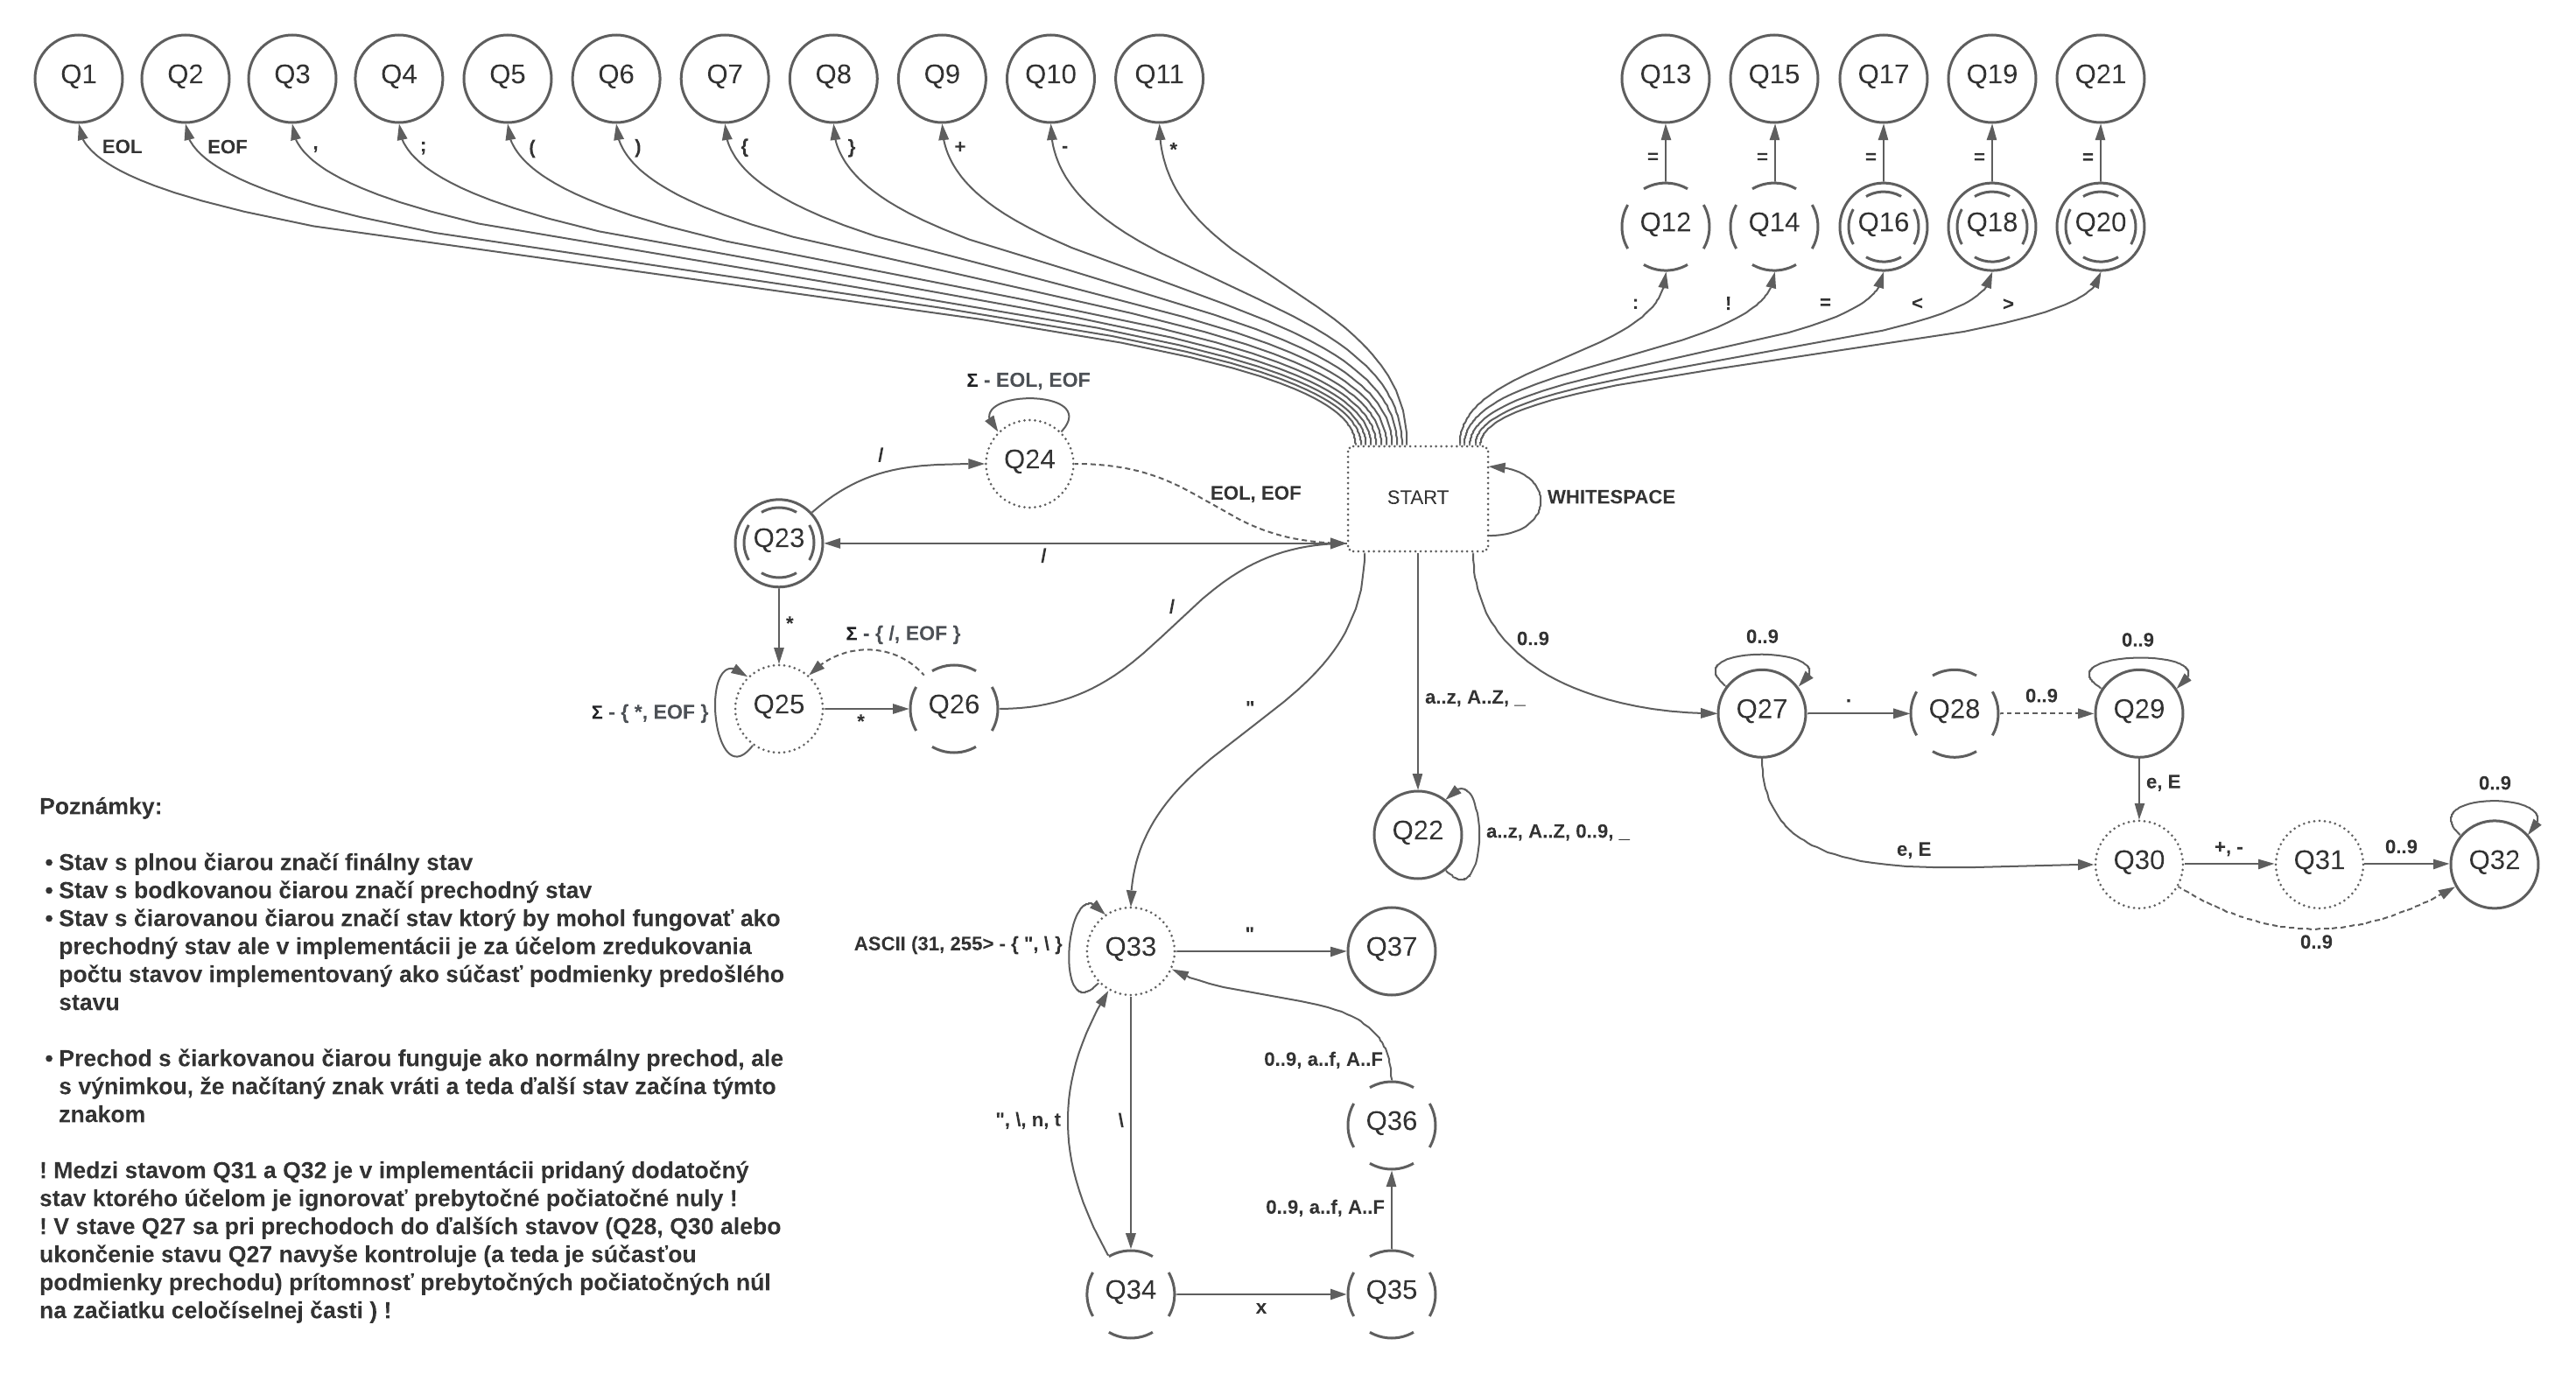
\includegraphics{automat.png}}
            \end{figure}
        \end{center}
    \end{landscape}
\newpage
    \begin{center}
        \section{LL-Gramatika}
            \begin{figure}[h]
                \centering
                \scalebox{0.39}{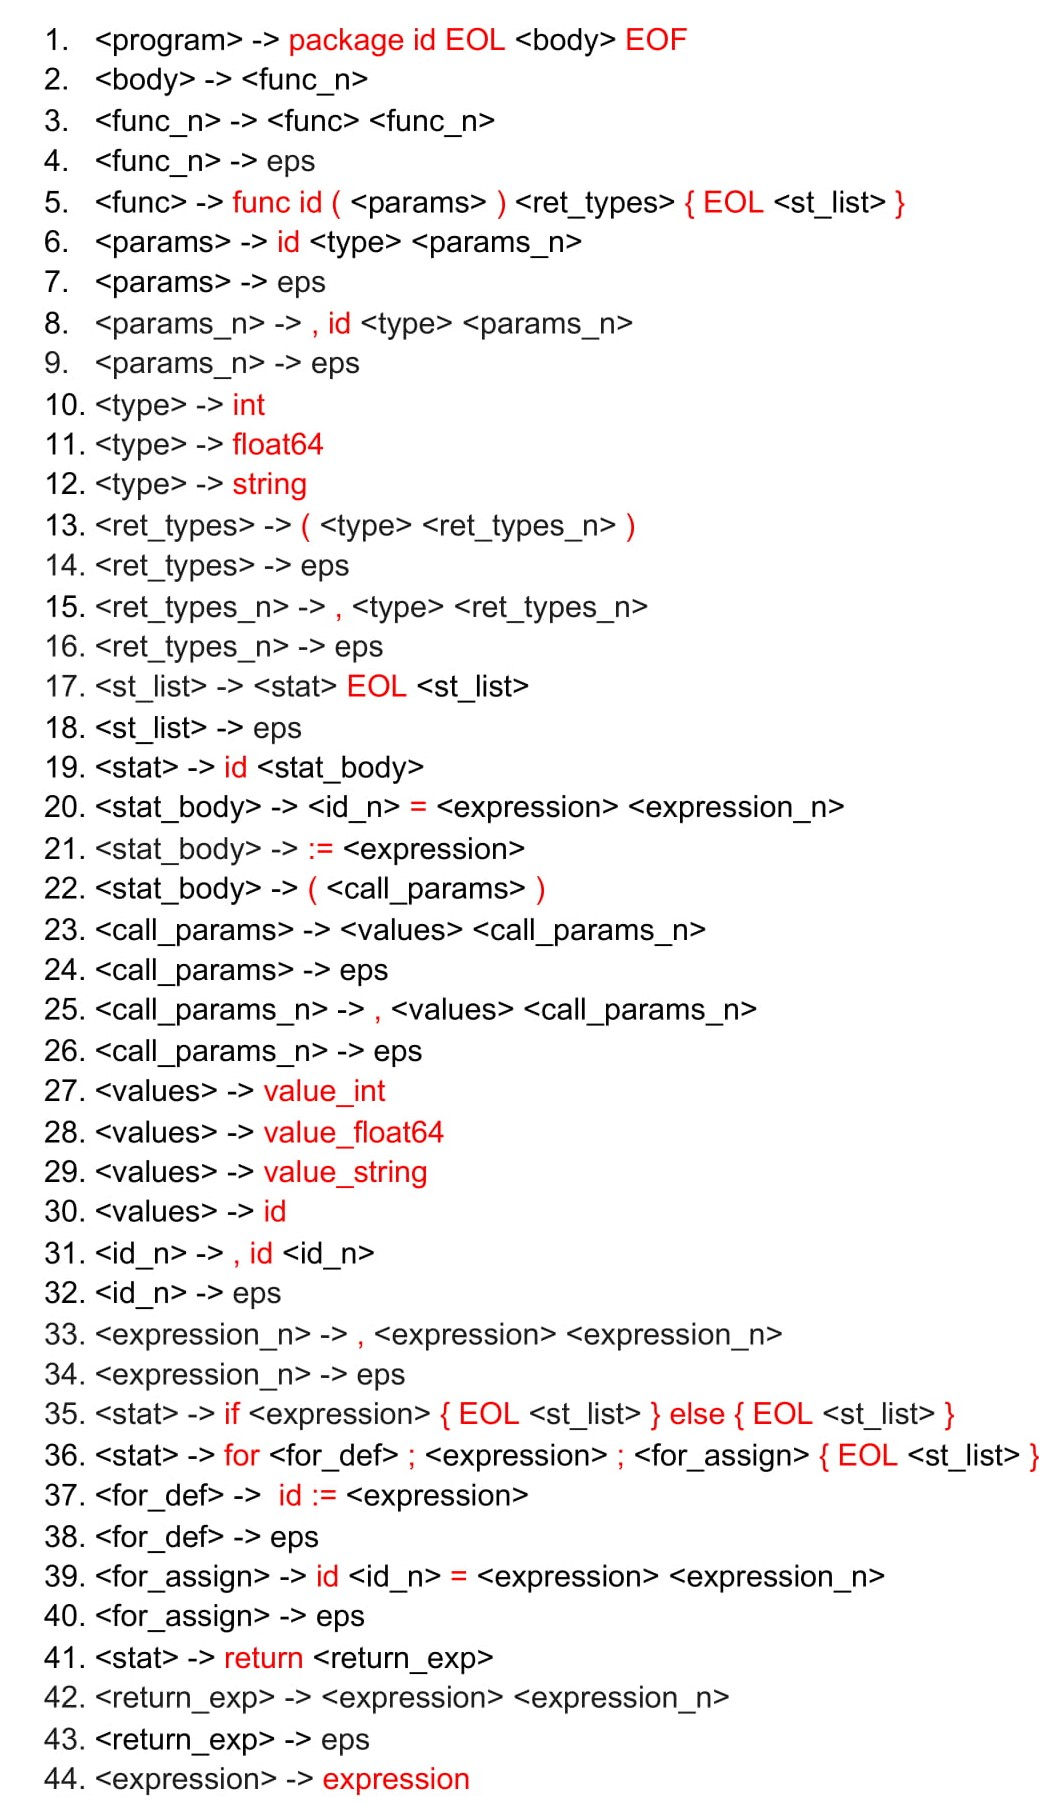
\includegraphics{pravidla.jpg}}
            \end{figure}
    \end{center}
\newpage
    \begin{center}
        \section{Pravidlá pre výrazy}
            \begin{figure}[h]
                \centering
                \scalebox{0.8}{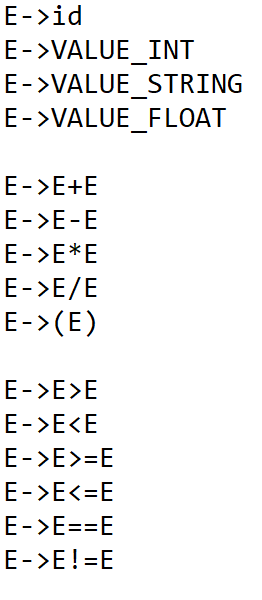
\includegraphics{exp_pravidla.png}}
            \end{figure}
    \end{center}
\newpage
    \begin{landscape}
        \begin{center}
            \section{LL-Tabuľka}
                \begin{figure}[h]
                    \scalebox{0.5}{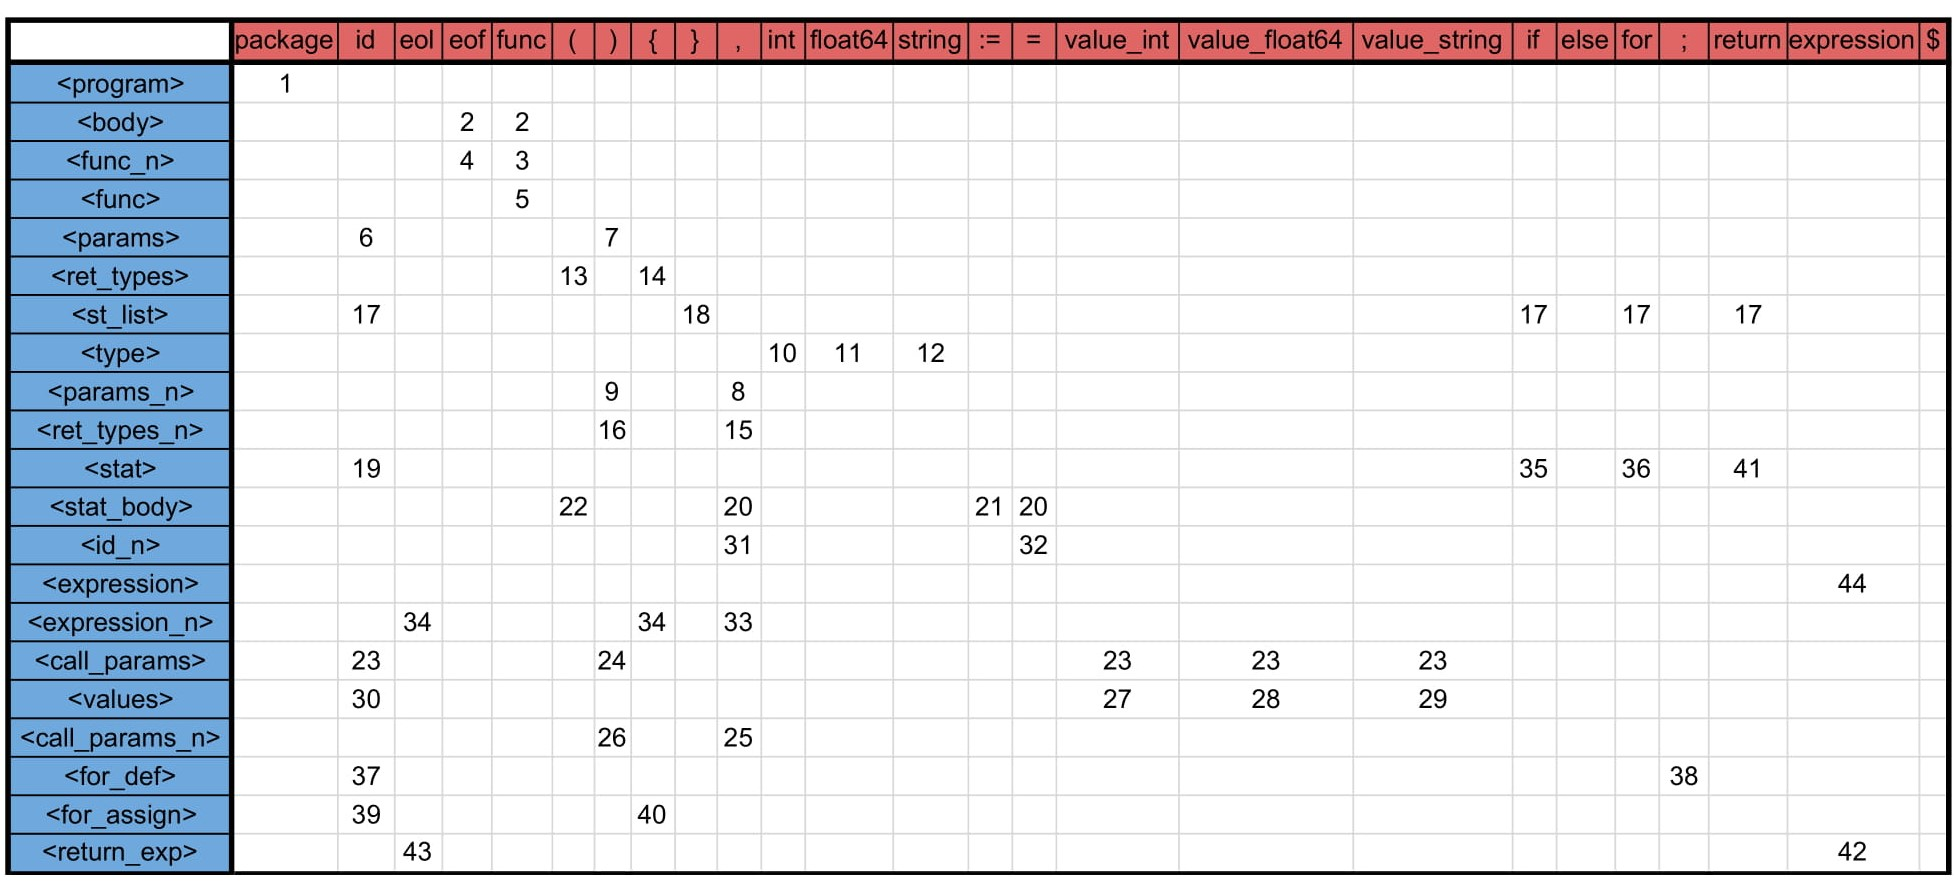
\includegraphics{LL_tabulka.jpg}}
                \end{figure}
        \end{center}
    \end{landscape}
\newpage
    \begin{landscape}
        \begin{center}
            \section{Precedenčná tabuľka}
                \begin{figure}[h]
                    \scalebox{0.6}{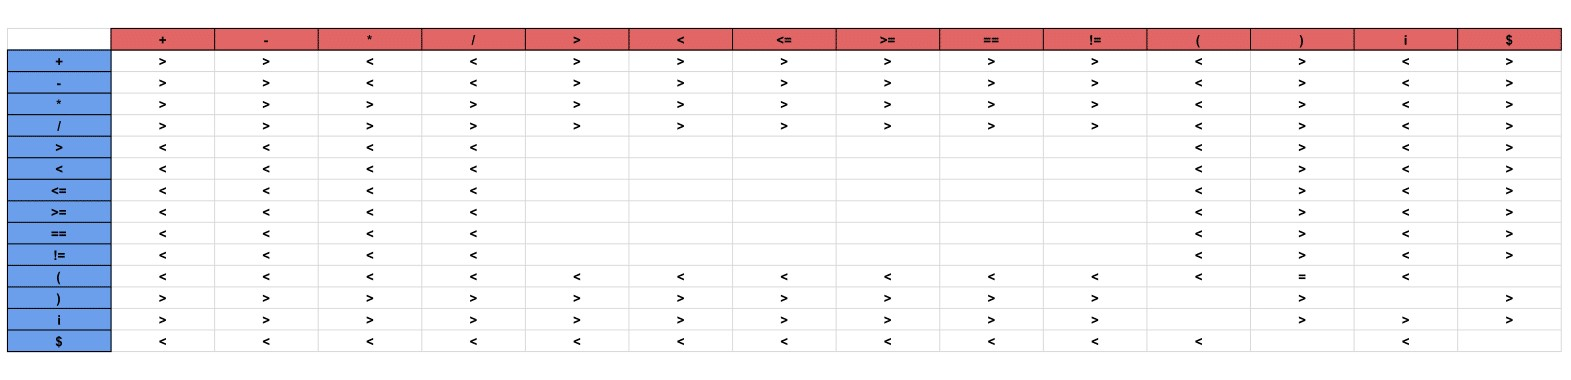
\includegraphics{precedencna.jpg}}
                \end{figure}
        \end{center}
    \end{landscape}

\end{document}
